\documentclass[a4paper]{article}
\usepackage[utf8]{inputenc}
\usepackage[russian]{babel}
\usepackage{listings}
\usepackage[a4paper]{geometry}
\usepackage{indentfirst}
\usepackage{graphicx}
\usepackage{caption}
\usepackage{float}
\usepackage{amssymb}
\usepackage{physics}

\begin{document}

\title{Отчёт по курсу <<Высокопроизводительные параллельные вычисления на кластерных системах>>.}
\author{Владислав Соврасов\\ аспирант гр. 2-о-051318}
\date{}
\maketitle

\section{Постановка задачи}

Требуется получить эффективную параллельную версию солвера MIDACO (http://www.midaco-solver.com), которая
бы эффективно работала как на распределённых системах, так и на системах с общей паматью.

MIDACO (Mixed Integer Distributed Ant Colony Optimization) предназначен для решения
глобальной оптимизации как с дискретными, так и с непрерывными параметрами.

Будем рассматривать задачу глобальной оптимизации в неперрывном многомерном пространстве:
\begin{displaymath}
\label{task}
\varphi(y^*)=\min\{\varphi(y):y\in D\},D=\{y\in \mathbf{R}^N:a_i\leqslant x_i\leqslant{b_i}, 1\leqslant{i}\leqslant{N}\}
\end{displaymath}

\section{Реализация}



\section{Результаты}

\begin{figure}[H]
  \center
  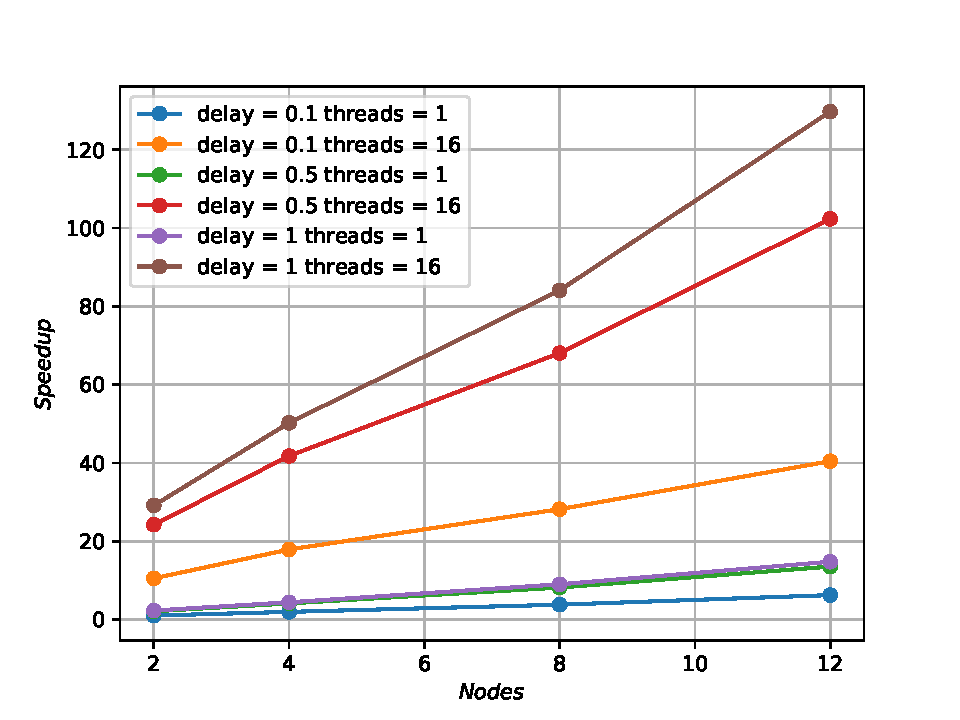
\includegraphics[width=0.75\textwidth]{gpu_mpi/gklsh4d/speedup_nodes.pdf}
  \caption{}
  \label{fig:}
\end{figure}

\section{Исходный код}
\lstinputlisting[language=C++, numbers=left]{../src/midaco_mpi.cpp}

\end{document}
